\documentclass[12pt,reqno,oneside]{amsart}
\usepackage[style=numeric, backend=biber]{biblatex}
\usepackage{graphicx}
\theoremstyle{plain}
\newtheorem{Theorem}{Theorem}[section]
\newtheorem{Assumptions}{Assumption}
\newtheorem{TheoremCited}{Theorem}[section]
\newtheorem{Lemma}{Lemma}[section]
\newtheorem{Proposition}{Proposition}[section]
\newtheorem{Corollary}{Corollary}[section]
\newtheorem*{Theorem*}{Theorem}
\newtheorem*{Lemma*}{Lemma}
\newtheorem*{Proposition*}{Proposition}
\newtheorem*{Corollary*}{Corollary}
\newtheorem*{MainTheorem*}{Theorem \ref{main_theorem}}
\theoremstyle{definition}
\newtheorem{Definition}{Definition}[section]
\newtheorem*{Definition*}{Definition}
\theoremstyle{remark}
\newtheorem{Remark}{Remark}[section]
\newtheorem*{Remark*}{Remark}
\newtheorem{Claim}{Claim}[section]
\newtheorem*{Claim*}{Claim}
\numberwithin{equation}{section}
\renewcommand{\H}{{\mathbb{H}^n}}
\newcommand{\Ga}{{\Gamma}}
\newcommand{\I}[1]{{#1^{i}}}
\renewcommand{\O}[1]{{#1^{o}}}
\newcommand{\PH}{{\partial \H}}
\newcommand{\IG}{{\Ga^+}}
\newcommand{\OG}{{\Ga^-}}
\newcommand{\tf}{{\tilde{f}}}
\newcommand{\e}{{\varepsilon}}
\renewcommand{\L}{\Lambda}
\newcommand{\below}[2]{{\mathop{#1}\limits_{#2}}}
\newcommand{\thin}[1]{{{#1}}}
\newcommand{\thick}[1]{{{#1}}}
\newcommand{\con}[1]{{{#1}^*}}
\newcommand{\ang}[1]{{\theta(#1)}}
\newcommand{\diam}{{\text{diam}}}
\newcommand{\LL}{\mathcal{L}}
\bibliography{hyperbolicisometries}

\begin{document}

\title[Characterizations of Hyperbolic Isometries]{Hyperbolic Isometries via Horospheres and Equidistant Surfaces}
\author{QIANG GAO}

\address{Department of Mathematics, Sun Yat-Sen University, 510275, Guangzhou, P. R. China}
\email{ gaoqiangks@outlook.com}
\thanks{The	author is partially supported by NSFC, No: 11771456.  }


\begin{abstract}
	Let $\H$ be the $n$-dimensional hyperbolic space.  In this paper, we prove the
	following results. (I) An injective map $f: \H\mapsto \H$ is an isometry if and
	only if it preserves horospheres.  (II) An injective map $f:\H\mapsto\H$ is an
	isometry if and only if it preserves $r$-equidistant surfaces. We do not
	assume continuity in these results.

\bigskip
\noindent AMS Mathematics Subject Classification (2010): 30C35; 51M09;

\medskip

\noindent Keywords: M\"{o}bius transformation, hyperbolic geometry, horosphere,
equidistant surface.
\end{abstract}


\maketitle

\section{Introduction}
Let $\H$ be the $n$-dimensional hyperbolic space and $\mathbb{D}^n$ be the unit
ball model of $\H$.  The isometries of $\H$ are the
M\"{o}bius transformations that restrict to well defined maps on $\H$.  There
have been many theorems on characterizations of isometries of $\H$.  The
following results are known.
\begin{Theorem}[\cite{Jeffers2000Lost}] \label{geodesic_preserving}
	Suppose that $f:\H \mapsto \H$ is a bijection that preserves
	geodesics. Then $f$ is an isometry.
\end{Theorem}
\begin{Theorem}[\cite{Li09}]
	Suppose that $f: \H\mapsto\H$ is a bijection.  Then $f$ is an isometry if and
	only if $f$ is triangle domain preserving.
\end{Theorem}
\begin{Theorem}[\cite{Shi06}]
	Suppose that $f:\mathbb{D}^2\mapsto \mathbb{D}^2$ is a continuous bijection.
	Then $f$ is M\"{o}bius if and only if $f$ preserves Lambert quadrilaterals
	in $\mathbb{D}^2$.
\end{Theorem}
\begin{Theorem}[\cite{LiWangFundamental2016}]
	Suppose that $f : \mathbb{D}^n \mapsto \mathbb{D}^n $ is injective and maps
	any r-hyperplane into some r-hyperplane for some positive integer $r<n$.
	Then it is an isometry or a composition of an isometry and an affine
	transformation under the Klein model if and only if $f$ is non-degenerate.  
\end{Theorem}
For more such kind of rigidity results, one can see \cite{BeardonMinda2002sphere},\cite{chupin99},\cite{Gibbons1979Circle},\cite{Li09},\cite{huangwangwang2010isometries} and \cite{Shi08}.\par
Now we recall some basic definitions in hyperbolic geometry.  We use the upper
half space model of $\H$ unless otherwise stated.  For any point $p \in \H$, we
denote $p$ by $(x,y) \in \mathbb{R}^{n-1}\times \mathbb{R}^+$.
\begin{Definition}
	A geodesic plane is a vertical Euclidean plane or a Euclidean hemisphere
	that orthogonally intersects the $x$-plane.
\end{Definition}
\begin{Definition}
	An equidistant surface is a surface equidistant from a geodesic plane. An
	$r$-equidistant surface is an equidistant surface that is at the distance $r$
	from a geodesic plane.
\end{Definition}	
\begin{Definition}
	An $r$-hypercycle is a curve that lies on a geodesic 2-plane and that is
	$r$-equidistant from a geodesic.  It is also called an $r$-equidistant
	curve.
\end{Definition}
\begin{figure}[]
	\centering
	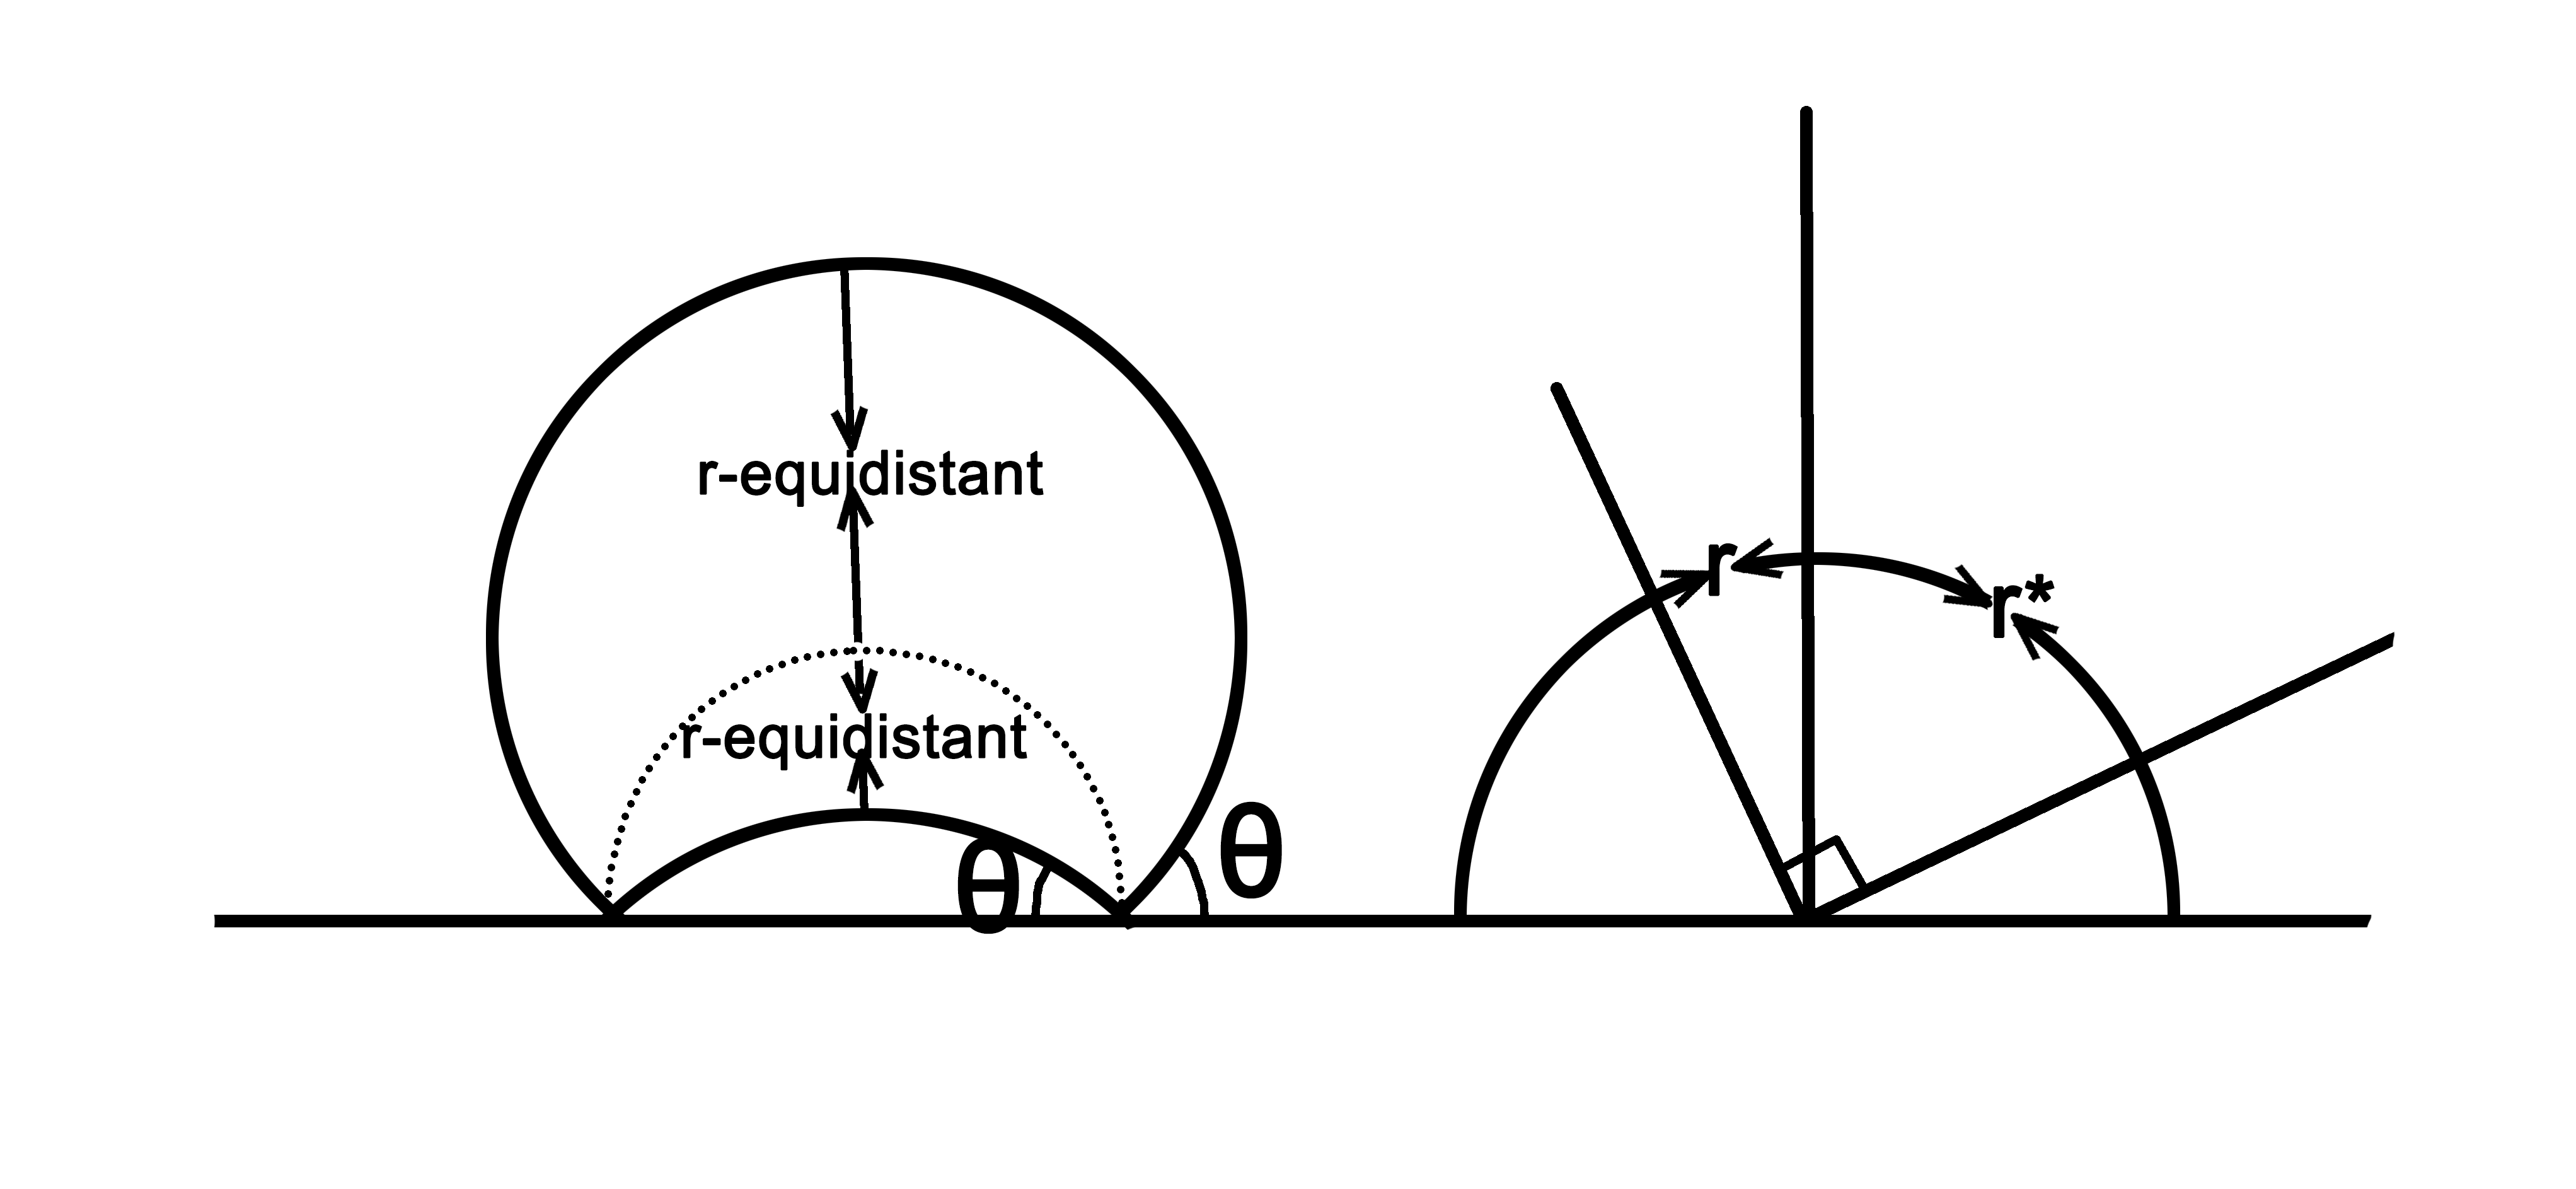
\includegraphics[scale=0.35]{0.png}
	\caption{Equidistant surfaces}
	\label{plane_horosphere_equidistant}
\end{figure}
\begin{Definition}
	A horosphere $\Ga$ is either a horizontal plane or a Euclidean sphere in $\H$ that is tangent to the $x$-plane.  The point $\Ga \cap \PH$ is called the center of the horosphere.
\end{Definition}
\begin{Definition}
	Let $f: \H\mapsto \H$. We way that $f$ preserves horospheres if for any
	horosphere $\Ga$, $f(\Ga)$ is a horosphere, and we say that $f$ preserves
	$r$-equidistant surfaces if for any $r$-equidistant surface $\Ga$, $f(\Ga)$
	is an $r$-equidistant surface.
\end{Definition}
It's well-known that a Euclidean sphere or a Euclidean plane that intersects the
$x$-plane with an angle $\theta$ is an $r(\theta)$-equidistant surface where
\begin{equation}
	r(\theta)=\ln(\frac{1+\cos\theta}{\sin\theta}),
\end{equation}
and each $r$-equidistant surface can obtained this way.  See Figure
\eqref{plane_horosphere_equidistant}.
For any $r>0$, let $\con{r}$ denote the unique number satisfying
\begin{equation}\label{def_rstar}
	\theta(r)+\theta(\con{r})=\frac{\pi}{2}.
\end{equation}
If $\Ga$ is a horosphere, then we denote the interior of $\Ga$ by $\Ga^+$ and
the exterior of $\Ga$ by $\Ga^-$.   If $\Ga$ is an $r$-equidistant surface,
$\Ga$ divides the hyperbolic space $\H$ into two parts.  One of the two parts
contains the geodesic plane that shares the same boundary with $\Ga$.  We call
this part the thick part of $\Ga$ and call the other part the thin part of
$\Ga$.  Denote the thick part of $\Ga$ by $\Ga^+$ and the thin part by $\Ga^-$.
Now we state our main results.
\begin{Theorem}\label{MainTheoremA}
	Let $f:\H\mapsto \H$ be an injective map.  Then $f$ is an isometry if and only if
	it preserves horospheres.
\end{Theorem}
\begin{Theorem}\label{MainTheoremB}
	Let $f:\H\mapsto\H$ be an injective map.  Then $f$ is an isometry if and only
	there exists a constant $r>0$ such that $f$ preserves $r$-equidistant
	surfaces.
\end{Theorem}



\section{Proof of Theorem \eqref{MainTheoremA}}
\begin{Lemma}\label{iioo}
	Let $\Ga$ be a horosphere. Then $f$ maps the interior of $\Ga$ into the
	interior of $f(\Ga)$ and maps the exterior of $\Ga$ onto the exterior of
	$f(\Ga)$.
\end{Lemma}
\begin{proof}
	%By an isometry, assume that $\Ga=\{x\in \H\mid x_n=1\}$.  
	Let $p \in \OG$.  Let $\Ga'$ be a horosphere that contains $p$ and is
	tangent to $\Ga$.  Then $f(\Ga')$ is tangent to $f(\Ga)$ at $f(p) \in \H$.
	Therefore, $f(p) \in f(\Ga)^-$.  To show that $f$ maps the interior of $\Ga$
	into the interior of $f(\Ga)$, we show that $f|_\OG$ is surjective.  
	Suppose that $\Ga=f(\Ga)=\{(x,y)\in \H \mid y=1\}$.  For any point $p \in
	\Ga$, let $\Ga_p$ denote the unique horosphere that is tangent to $\Ga$
	at the point $p$.
	Then
	\begin{equation}
		\Ga^-=\below{\cup}{p\in \Ga}\Ga_p=\below{\cup}{p\in \Ga}f(\Ga_p)=f(\Ga)^-
	\end{equation}
	Then $f|_{\Ga^-}: \Ga^- \mapsto f(\Ga)^-$ is surjective.  Since $f$ is
	injective, $f$ maps $\Ga^+$ into $f(\Ga)^+$.
\end{proof}
\begin{Lemma}
	The map $f$ is surjective.
\end{Lemma}
\begin{proof}
	Let $q \in \H$.  Take two disjoint horospheres $\Ga_1$ and $\Ga_2$ such that
	$\Ga_1\cap \PH \neq \Ga_2 \cap \PH$.  If $q \in f(\Ga_1) \cup f(\Ga_2)$, then we finish the proof.  Otherwise, observe that $f(\Ga_1)^+ \cap
	f(\Ga_2)^+=\emptyset$.  Therefore, $q \in f(\Ga_1)^-$ or $q\in f(\Ga_2)^-$.
	In either case, the point $q$ has a preimage since $f|_{\Ga^-} : \Ga^-
	\mapsto f(\Ga)^-$ is surjective for any horosphere $\Ga$.
\end{proof}
\begin{Lemma}
	The map $f$ extends to a homeomorphism between $\overline{\H}$.
\end{Lemma}
\begin{proof}
	We first show that $f$ induces a homeomorphism between $\PH$.  Let $p~\in~\PH$.
	Let $\Ga$ be a horosphere centered at $p$.  Define $\tf(p)$ to be the center
	of $f(\Ga)$.  By Lemma \eqref{iioo}, $\tf(p)$ is independent of the choice
	of $\Ga$ and the map $\tf$ is injective.  Now we show that $\tf$ is
	continuous.  Let~$p_n\in \PH$ and $p_n\to p$.  Suppose to the contrary that
	$\tf(p_n)\to q \neq \tf(p)$.  Assume that $p=\tf(p)=\infty$ and
	$\Ga=\{(x,y)\in \H \mid y=1\}$.  Let $\{\Ga_n\}$ be the horosphere centered
	at $p_n$ and tangent to $\Ga$.  Up to a subsequence, assume that $\{\Ga_n\}$
	are pairwise disjoint.  Observe that $f(\Ga_n)$ is a Euclidean sphere of
	unit diameter.  It's clear that $\tilde{f}(p_n)$ doesn't accummulate to a finite point, which leads to a contradiction.
	There, $\tilde{f}$ is continuous, and thus is a homeomorphism between $\PH$.
	Let $p_n \in \H$ and $p_n \to p\in \PH$.  For each $p_n$, take a horosphere $\Ga_n$
	centered at $p$ and through $p_n$.  Up to a subsequence, suppose that
	$\Ga_{n+1} \subset \Ga_n^+$.  Now we show that $f(\Ga_n) \to f(p)$.
	Suppose to the contrary that $f(\Ga_n) \to \L$ for some horosphere $\L$
	centered at $f(p)$.  Then $f(\below{\cup}{n}\Ga_n^-) \subset \L^-$, which
	leads to a contradiction.  Therefore, $f(p_n) \to f(p)$.
	\par
	Now we show that $f$ is continuous in $\H$.
	Let $p\in \H$ and $a,b \in \PH$.  Without loss of generality, assume that
	$a$ is at the origin, $b=\infty$ and $p=(0,0,\cdots,1)$.  For each
	$p_t=(0,0,\cdots,t)$, let $\Ga_a^t$ be the horosphere centered at $a$ and
	through $p_t$.  Let $\Ga_b^t=\{(x,y)\in \H\mid y=t\}$.  
	\begin{figure}[]
		\centering
		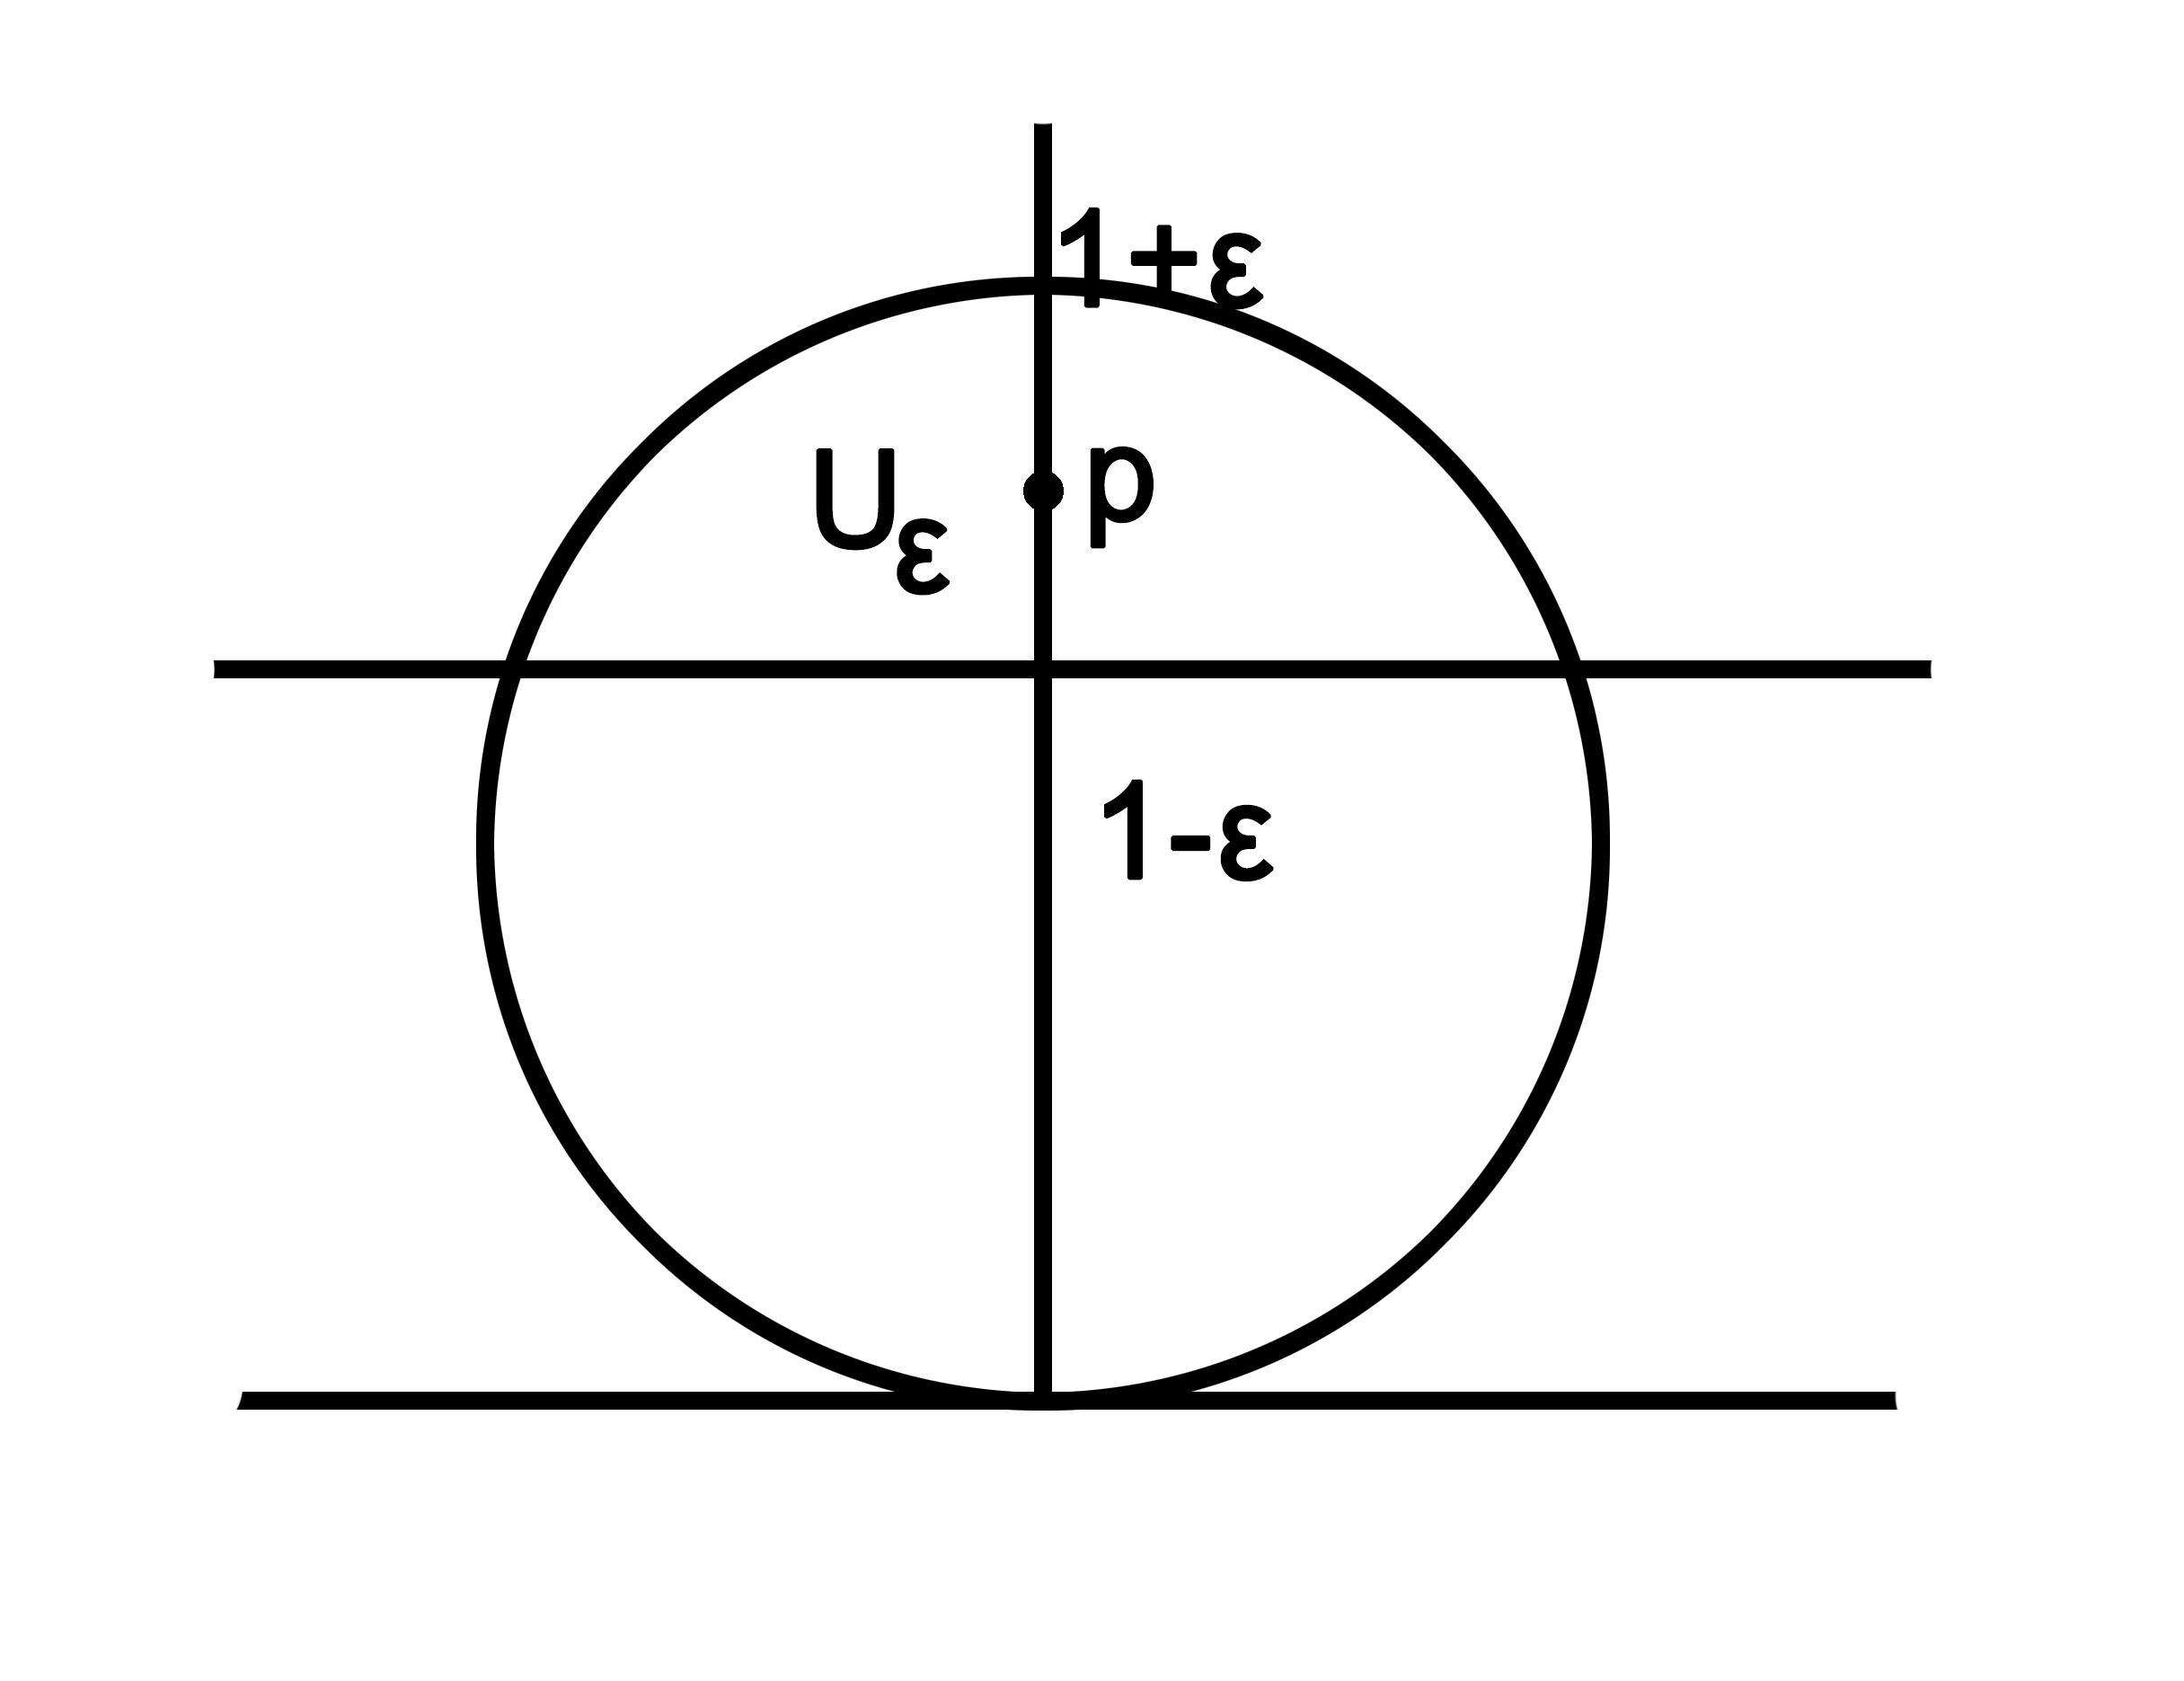
\includegraphics[scale=0.35]{3.png}
		\caption{}
		\label{neighborhood}
	\end{figure}
	Then for any $\e>0$,
	$\Ga_a^{1+\e}$ and $\Ga_b^{1-\e}$ bound a neighborhood $U^\e$ of $p$.  See
	Figure \eqref{neighborhood}.  Let
	$\e\to 0$.  There holds 
	\begin{equation}
		\below{\cap}{\e\to 0} f(U_\e)=f(\below{\cap}{\e\to0}U_\e)=f(p)
	\end{equation}
	Therefore, $f$ is continuous.  By invariance of domain, $f$ is a
	homeomorphism between $\overline{\H}$.
\end{proof}
\begin{proof}[Proof of Theorem \eqref{MainTheoremA}]
	Let $a,b \in \PH$. Let $\gamma$ be the geodesic connecting $a$ and $b$. Then
	$\gamma$ can be characterized as
	\begin{equation}
		\begin{split}
			\{p \in \H \mid &\text{There exist two tangent horospheres } \Ga_a\text{ and } \Ga_b \\
							&\text{centered at }a \text{ and } b \text{ respectively such that }  p=\Ga_a \cap \Ga_b \}
		\end{split}
	\end{equation}
	Since $f$ is a homeomorphism and
	horosphere-preserving, $f$ is geodesic-preserving.  By Theorem
	\eqref{geodesic_preserving}, $f$ is an isometry.
\end{proof}
\section{Proof of Theorem \eqref{MainTheoremB}}
The proof of Theorem \eqref{MainTheoremB} is quite similar to the proof of Theorem \eqref{MainTheoremA}.
\begin{Lemma} \label{thinthick}
	Let $\Ga$ be an $r$-equidistant surface.  Then $f$ maps the thin part of $\Ga$
	onto the thin part of $f(\Ga)$ and maps the thick part of $\Ga$ into the
	thick part of $f(\Ga)$.
\end{Lemma}
\begin{proof}
	Let $p \in \thin{\Ga^-}$.  Then there exists an $r$-equidistant surface $\Ga'$
	containing $p$ and tangent to $\Ga$.  Then $f(\Ga')$ is tangent to $\Ga$,
	and thus, $f(p)$ lies in the thin part of $f(\Ga)$.  Observe that for any point $p \in \Ga$, there exists a unique $r$-equidistant surface lying in $\Ga^-$ and  tangent to $\Ga$ at $p$.  Let $\Ga_p$ denote this $r$-equidistant surface.  Then
	\begin{equation}
		\Ga^-=\below{\cup}{p\in \Ga}\Ga_p=\below{\cup}{p\in \Ga}f(\Ga_p)=f(\Ga)^-
	\end{equation}
	Therefore $f|_{\Ga^-}$ is a surjective map from $\Ga^-$ to $f(\Ga)^-$.  Since $f$ is
	injective, $f$ maps $\Ga^+$ into $f(\Ga)^+$.
\end{proof}
\begin{Lemma} \label{f_surjective}
	The map $f$ is surjective.
\end{Lemma}
\begin{proof}
	If there exists a point $o \in \PH$ such that there exists a sequence of
	$r$-equidistant surfaces $\{\Ga_n\}$ satisfying
	\begin{enumerate}
		\item $o \in \thick{\Ga^+_{n+1}} \subset \thick{\Ga^+_n}$,\label{in_thick}
		\item $\Ga_n \to o$,\label{degenerate_surface}
		\item $f(\Ga_n) \to q$ for some $q \in \PH$.\label{deg_f_surface}
	\end{enumerate}
	Then by Lemma \eqref{thinthick}, $f$ is surjective on $\thin{\Ga_n^-}$ for
	each $n$, and thus, is a surjective map.   Therefore, we have only to show that
	such a point exists.  Suppose to the contrary.  For any point $p \in \PH$,
	take a sequence of $r$-equidistant surface $\{\Ga_{p,n}\}$
	such that $p \in \thick{\Ga^+_{p,n+1}}\subset \thick{\Ga^+_{p,n}}$ and
	$\Ga_{p,n} \to p$.  Suppose that condition \eqref{deg_f_surface} doesn't
	hold.  By Lemma \eqref{thinthick}, $\thick{f(\Ga_{p,n+1})^+}\subset
	\thick{f(\Ga_{p,n})^+}$.  Therefore, there exists an $r$-equidistant surface
	$\L_p$ such that $f(\Ga_{p,n}) \to \L_p$.  For two points $p\ne q$ and $n$
	large enough, there hold $\thick{\Ga^+_{p,n}}\subset \thin{\Ga_{q,n}^-}$ and
	$\thick{\Ga^+_{q,n}}\subset \thin{\Ga^-_{p,n}}$.  Then we have $\thick{\L_p^+} \subset
	\thin{\L^-_q}$ and $\thick{\L_q^+} \subset \thin{\L^-_p}$.  Specially,
	$\thick{\L_p^+}$ is disjoint from $\thick{\L_q^+}$.  Consider the unit
	ball mode.  Then each $\thick{\L_p^+}$ is of finite positive Euclidean
	measure.  However, this is impossible since there are uncountably many such
	$r$-equidistant surfaces and the sum of uncoutably many positive numbers must
	be $+\infty$.  Thus, the lemma follows.
\end{proof}
\begin{Lemma}
	The map $f$ extends to a homeomorphism between $\overline{\H}$.
\end{Lemma}
\begin{proof}
	We first show that $f$ extends naturally to the boundary.  Let $p \in \PH$.
	Take a sequence of $r$-equidistant surfaces $\{\Ga_n\}$ such that
	$p \in \thick{\Ga^+_{n+1}}\subset \thick{\Ga^+_n}$ and $\Ga_n \to p$. The limit of $f(\Ga_n)$ must be either a point or an $r$-equidistant surface.  Suppose the latter
	case holds and denote this limiting surface by $\L_p$.  Then $f$ maps
	$\thin{f(\Ga_n)^-}$ into $\thin{\L^-_p}$ for each $n$, and thus $f$ maps $\H$ into $\L^-_p$, which contradicts to Lemma
	\eqref{f_surjective}.  Therefore, $f(\Ga_n) \to q$ for some point $q \in
	\PH$. Define $f(p)=q$.  It's clear that $q$ is independent of
	the choice of $\{\Ga_n\}$ and $f|_\PH$ is injective.  Let $p \in \H$.  Take two $r$-equidistant surfaces
	$\Ga_1$ and $\Ga_2$ such that $p \in U_\e=\thick{\Ga^+_1} \cap \thick{\Ga^+_2}$ with
	$\diam(U_\e) < \e$.  Letting $\e \to 0$, then
	we have
	\begin{equation}
		\below{\cap}{\e\to0}f(U_\e)=f(\below{\cap}{\e\to0}U_\e)=f(p)
	\end{equation}
	Therefore, $f$ is continuous in $\H$.  Let $p \in \PH$ and $\overline{\H}
	\ni p_k \to p$.  Take a sequence of $r$-equidistant surfaces $\Ga_n$ such
	that $p \in \thick{\Ga^+_{n+1}}\subset \thick{\Ga^+_n}$ and $\Ga_n\to p$.  Then
	for each $n$,
	there exists a constant $K$ such that for any $k>K$, $p_k \subset \Ga_n^+$ and thus $f(p_k) \subset
	\thick{f(\Ga_n)^+}$.  Since $\thick{f(\Ga)^+_n} \to f(p)$, $f(p_k)\to f(p)$.
	Therefore, $f$ is a homeomorphism between $\overline{\H}$.
\end{proof}
\begin{Lemma}\label{f_geodesic_preserving}
	The map $f$ is geodesic-preserving.
\end{Lemma}
\begin{proof}
	We first show that $f$ preserves $\con{r}$-hypercycles.  Let $\Ga$
	be an $r$-equidistant surface.  Without loss of generality, assume that $\Ga$
	is a plane that forms an angle $\ang{r}$ with the $x$-plane.  Let $p \in
	\Ga\cap x$-plane.  Let $\Ga'\subset \Ga^+$ be a plane parallel to $\Ga$.  Then there's a
	unique $r$-equidistant surface $\L$ such that $\L$ contains $p$ and is tangent to both $\Ga$ and $\Ga'$.  See Figure \eqref{rstar}.
	\begin{figure}[h]
		\centering
		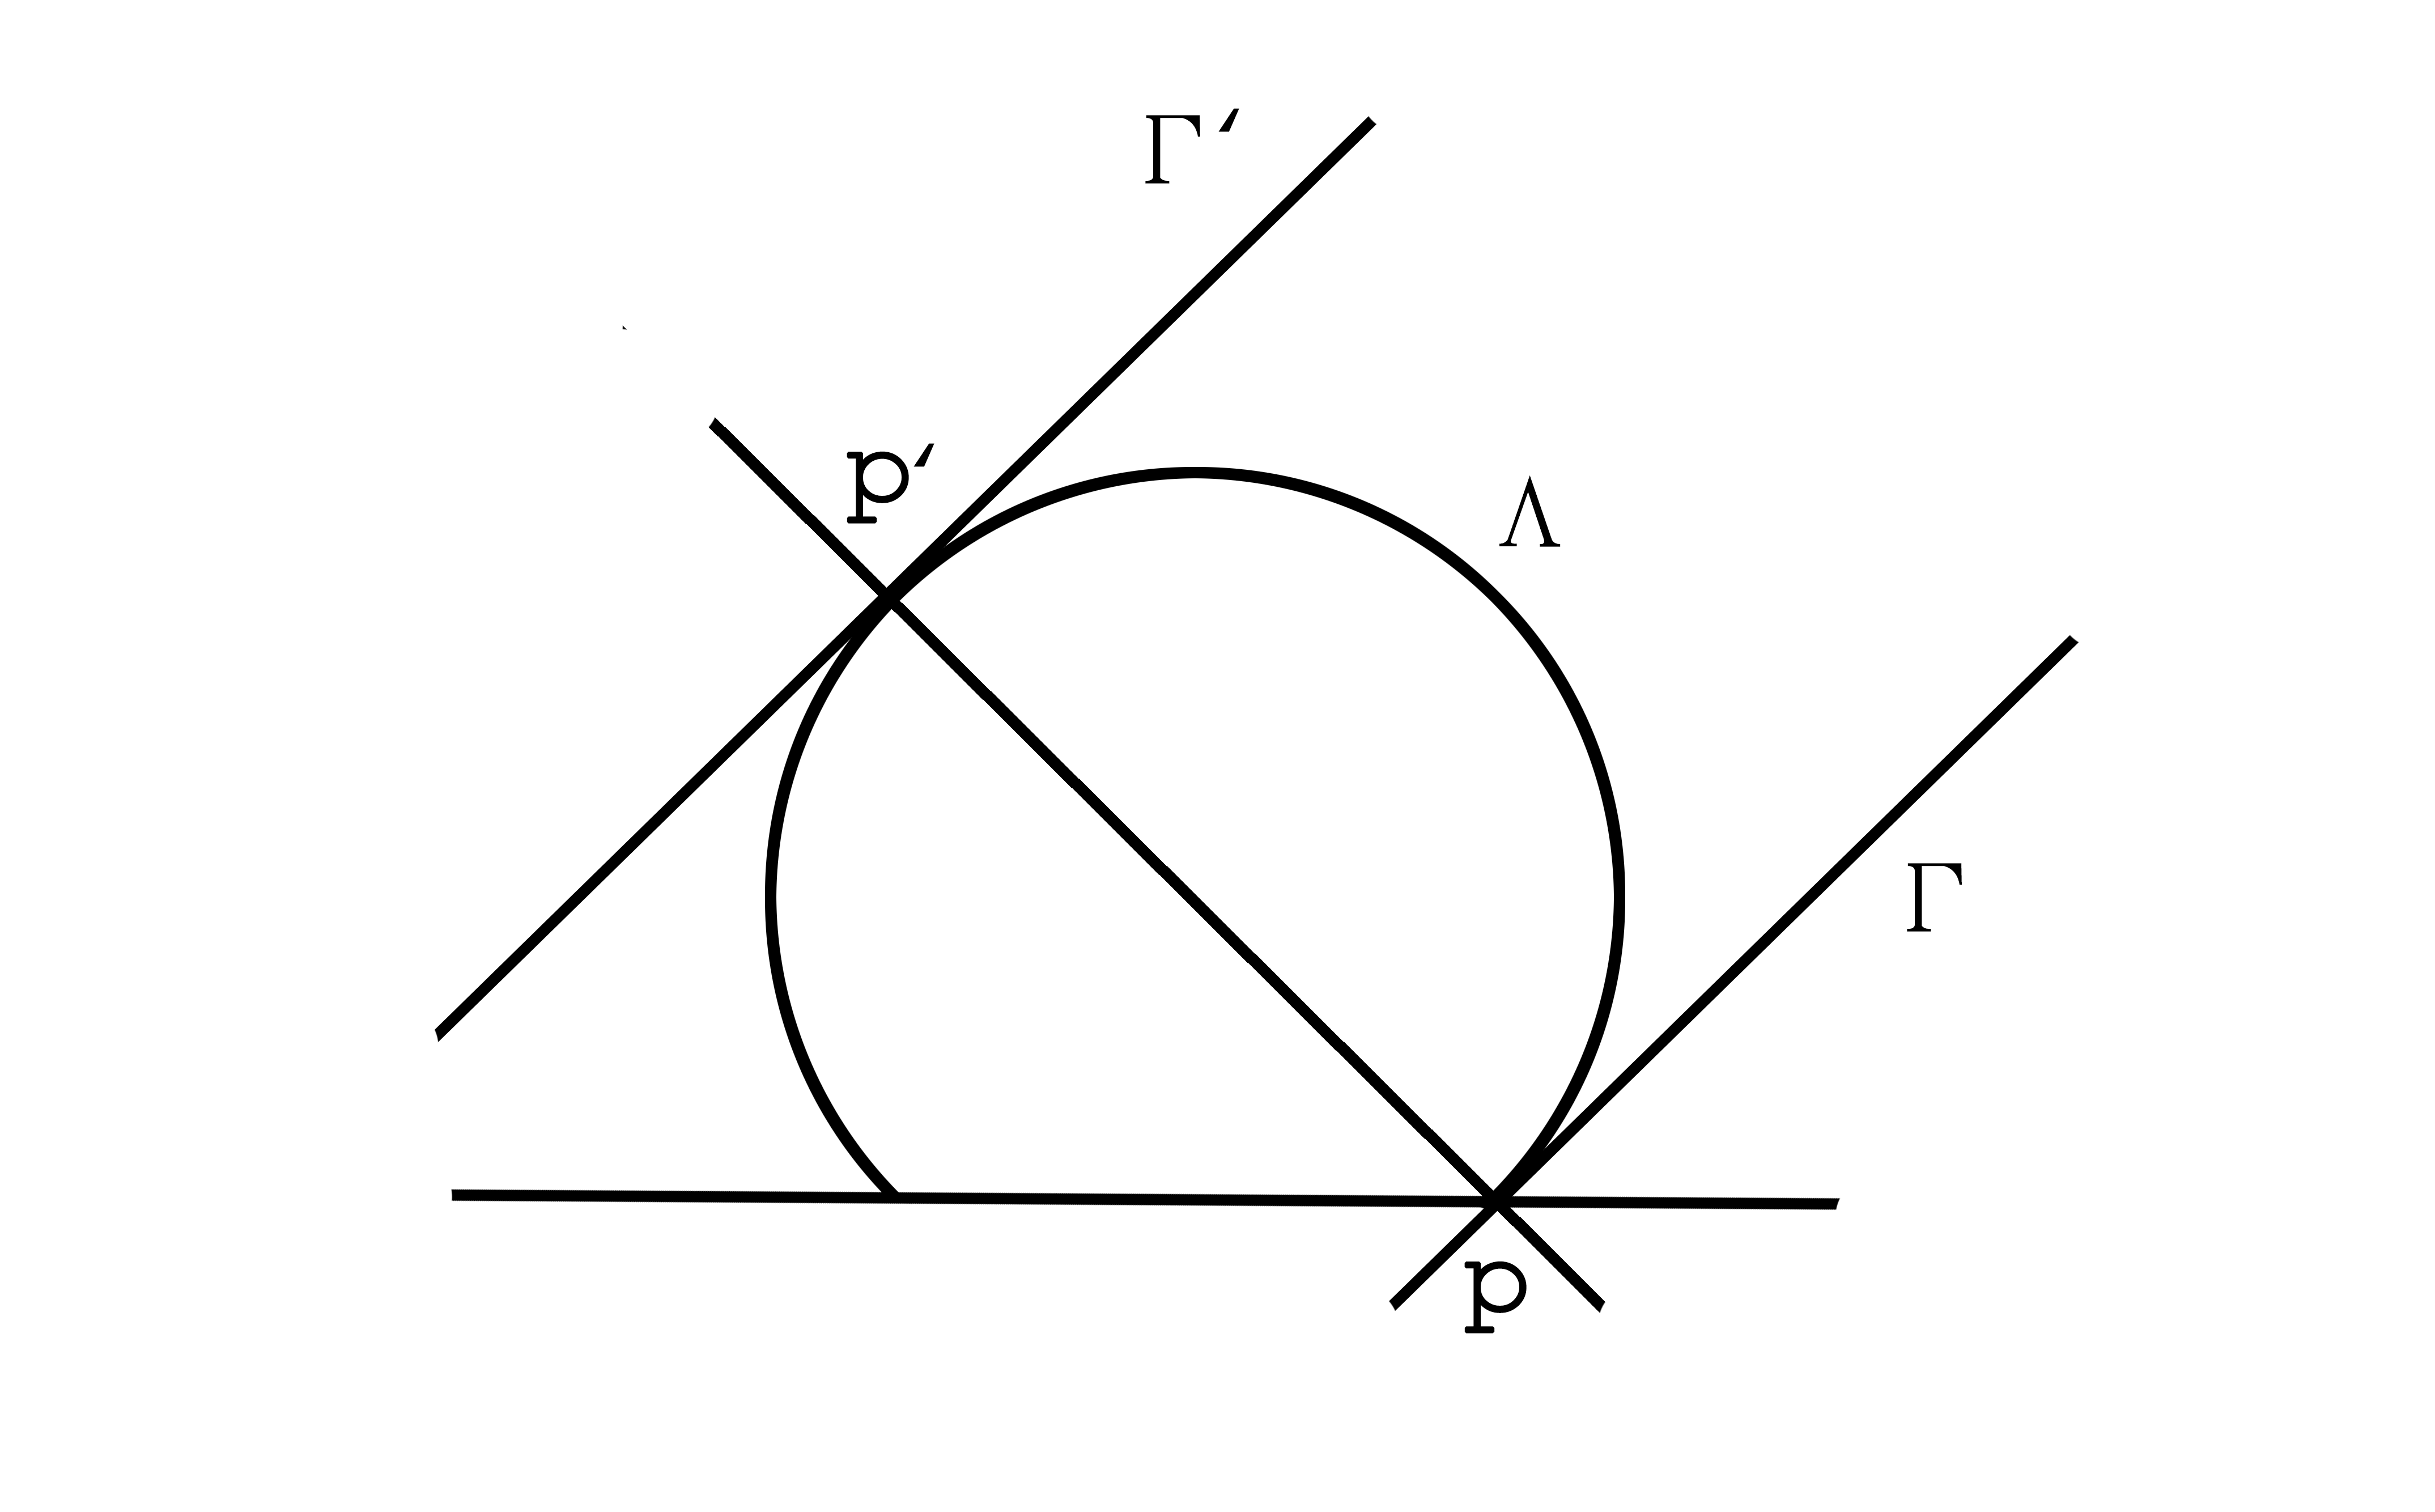
\includegraphics[scale=0.3]{1.png}
		\caption{Characterization of $r^*$-hypercycles}
		\label{rstar}
	\end{figure}
	Let $p'=\L\cap \Ga'$.  Moving $\Ga'$ to $\infty$ but still keep
	parallel to $\Ga$, then the orbit of
	$p'$ is an $\con{r}$-hypercycle, and each
	$\con{r}$-hypercycle can be obtained this way.  Consider the image of $\Ga$
	and $\Ga'$.  Suppose that $f(\Ga)\cap f(\Ga')=\infty$.  Then
	$f(\Ga)$ and $f(\Ga')$ are two disjoint planes.  By Lemma \eqref{thinthick},
	they must be parallel and $f(\L)$ is the
	$r$-equidistant surface lying between $\{f(\Ga),f(\Ga')\}$ and tangent to
	them.
	Since $f$
	is a homeomorphism and preserves $r$-equidistant surface, $f$ preserves
	$\con{r}$-hypercycles.  In addition, observe that, at the point $p$, there's a unique $r^*$-hypercycle connecting $\{p,\infty\}$ and perpendicular to $\Ga$, and it is exactly the orbit of $p'$. Denote this hypercycle by $\gamma$.  The above proof also shows that $f(\gamma)$ is the unique $r^*$-hypercycle connecting $\{f(p),\infty\}$ and perpendicular to $f(\Ga)$.  \par
	Suppose that $f(\infty)=\infty$.  Let $q \in \PH$ and $\L$ be an $r$-equidistant surface through $q$ such that
	$\infty~\in~\thin{\L^-}$.  Let
	$\LL$ be the unique $(n-2)$-plane through $q$ and tangent to
	$\L$, namely, $\LL=T_p\L~\cap~x\text{-plane}$.  The other $(n-2)$-plane parallel to $\LL$ and tangent to $\L$ is
	denoted by $\LL'$, and the tangent point is denoted by $q'$.  Let $\alpha$
	denote the geodesic through $q'$ and $\infty$.  Let $\beta$ denote the
	$r^*$-hypercycle through $q$ and perpendicular to $\L$.
	Then $o=\beta \cap \L \in \alpha$.  This can be seen from Figure
	\eqref{geodesic}.
	\begin{figure}
		\centering
		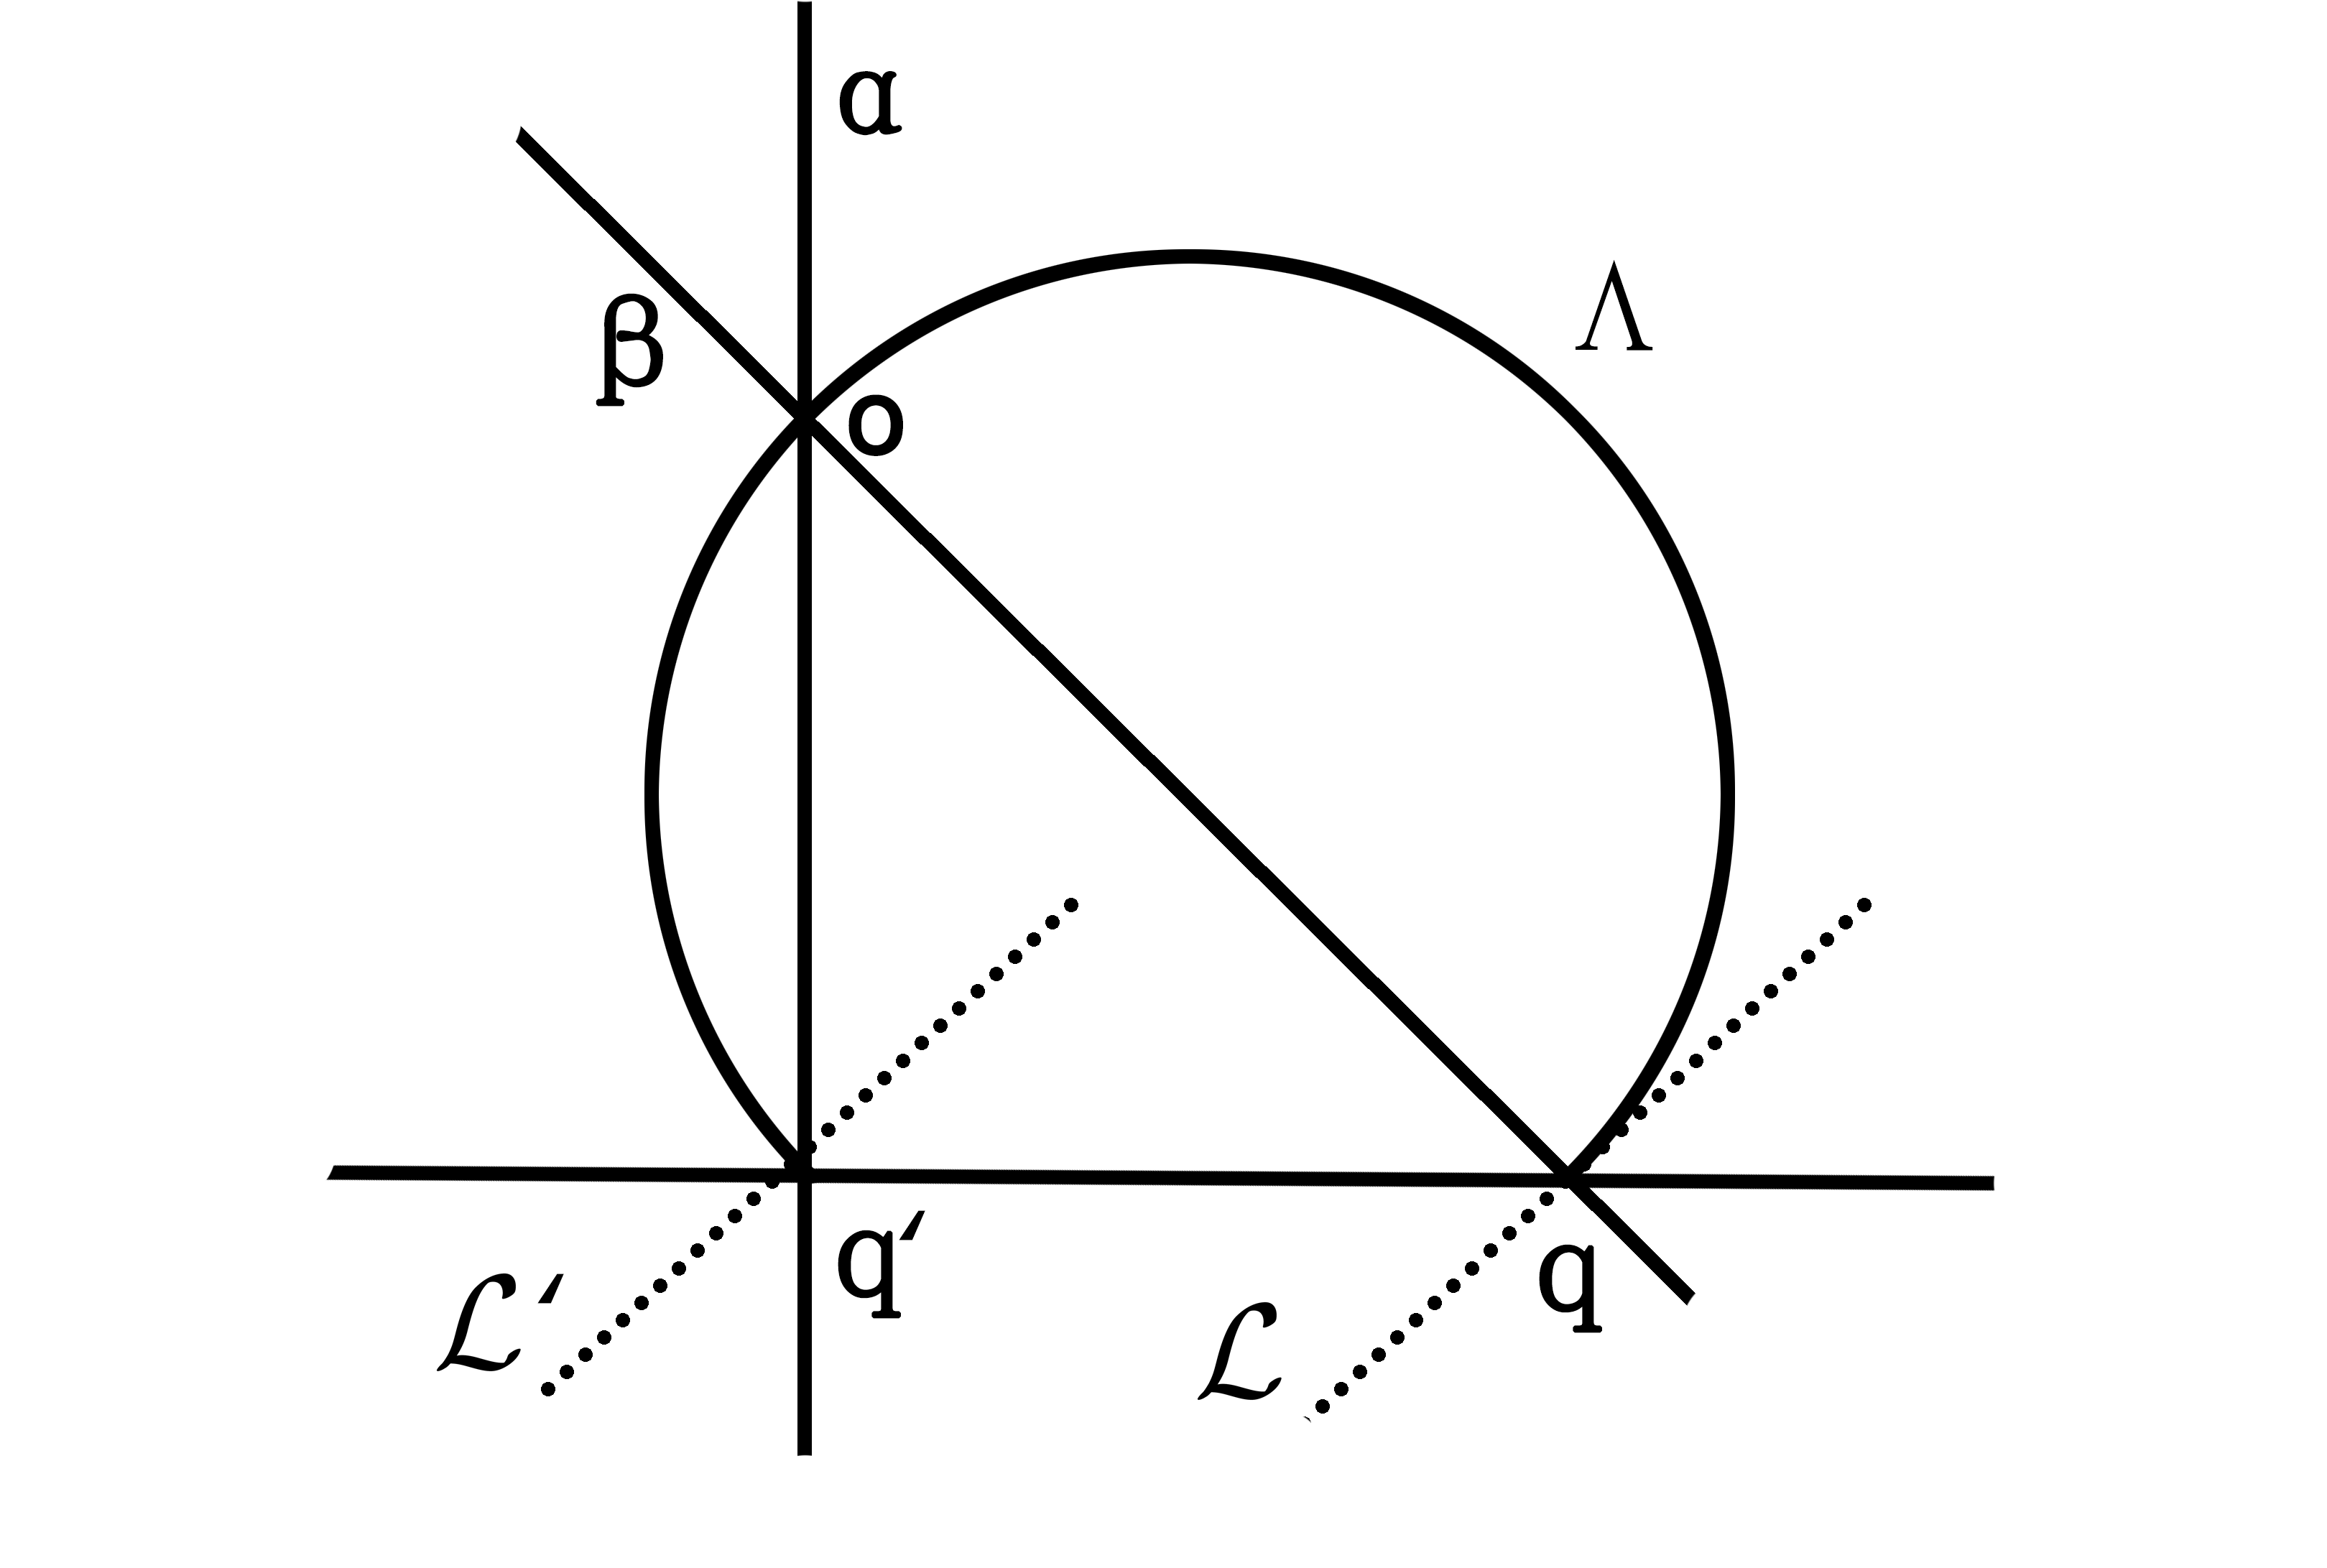
\includegraphics[scale=0.3]{2.png}
		\caption{Characterization of geodesics}
		\label{geodesic}
	\end{figure}
	Observe that $\L$ is uniquely determined by $\LL$ and $\LL'$.  Move $\LL$ to $\infty$ and keep it parallel to $\LL'$.  The orbit of $o$ is exactly the geodesic
	$\alpha$.  Since $f(\beta)$ is perpendicular to $f(\L)$, the orbit of $f(o)$ is the geodesic connecting $f(q')$ and $\infty$, and thus, $f$ preserves geodesics.
\end{proof}
\begin{proof}[Proof of Theorem \eqref{MainTheoremB}]
	This follows easily from Theorem \eqref{geodesic_preserving} and Lemma \eqref{f_geodesic_preserving}.
\end{proof}
\nocite{*}
\printbibliography
\end{document}
